\section{Ejercicio 3}

\subsection{Problema: Perdidos en los Pasillos}
El Pabell\'on 0+infinito, nuevamente remodelado, ahora tiene un disen\~o basado en un conjunto de M pasillos de distintas longitudes con intersecciones en donde se unen dos o m\'as pasillos. Es as\'i que puede modelarse como un grafo con pesos en los ejes, donde cada eje es un pasillo (de peso igual a la longitud del pasillo), y cada v\'ertices es una intersecci\'on o un extremo donde termina un pasillo sin unirse con ningu\'n otro. El decano junto con el director del Departamento de Computaci\'on, est\'an preocupados porque talvez existen ciclos en dicho grafo, lo que podr\'ia perjudicar a los alumnos al hacer que se pierdan buscando las aulas. Por tal motivo el decano decidi\'o clausurar los pasillos que sea necesario de manera tal que no queden ciclos en el grafo que representa al pabell\'on. El problema es que cuanto m\'as largo es un pasillo, m\'as costoso es clausurarlo. Disen\~ar un algoritmo de complejidad O(M log M ) para calcular la m\'inima suma posible de las longitudes de los pasillos que deber\'ian ser clausurados (eventualmente ninguno) para que no existan ciclos formados por tres o m\'as pasillos en el grafo que representa al pabell\'on. Se asegura que en toda instancia del problema el grafo que representa al pabell\'on es conexo.

\subsubsection{Explicacion del Problema}

    En este problema se tiene un edificio con pisos de longitud variable y portales que comunican pisos entre si. Por enunciado, este se puede representar como un grafo con pesos en sus ejes.
    
        %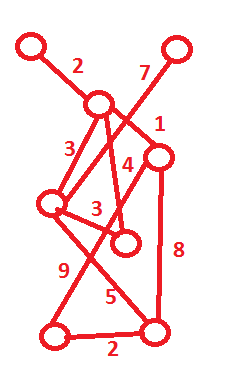
\includegraphics[scale=0.9]{imagenes/ejemploej3.png}\endl
        \begin{center}
\tikzset{main node/.style={circle,fill=white!20,draw,minimum size=0.75cm,inner sep=0pt},}
\begin{tikzpicture}
    
        \node[main node] (1) {1};
        \node[main node] (2) [right = 3.5cm of 1]  {$2$};
        \node[main node] (3) [above = 1.5cm of 1]  {$3$};
        \node[main node] (4) [right = 1.9cm of 3]  {$4$};
        
        \node[main node] (5) [above = 3.5cm of 2]  {$5$};
        \node[main node] (6) [left  = 1.8cm of 5]  {$6$};
        \node[main node] (7) [above = 2.5cm of 3]  {$7$};
        \node[main node] (8) [right = 3.5cm of 7]  {$8$};
    
        \path[draw,thick]
        (1) edge node {$2$} (2)
        (2) edge node {$5$} (3)
        (2) edge node {$8$} (5)
        (3) edge node {$3$} (4)
        (3) edge node {$7$} (8)
        (3) edge node {$3$} (6)
        (4) edge node {$4$} (6)
        (5) edge node {$1$} (6)
        (5) edge node {$9$} (1)
        (6) edge node {$2$} (7)
        (7) edge node {$2$} (8)
        ;
    
\end{tikzpicture}

    \\Ejemplo de grafo que representa el problema
\end{center}
        
    Lo que se quiere es eliminar (en el que caso de hubiera un ciclo) la menor cantidad de metros de pasillo posible (minima cantidad de peso total del ciclo) de manera tal que el grafo siga siendo conexo.
    
     %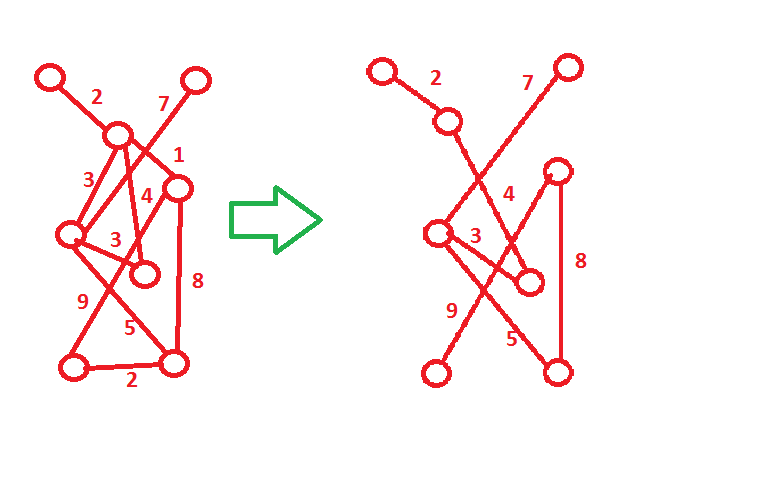
\includegraphics[scale=0.9]{imagenes/arbolgenmax.png}\endl
     \tikzset{main node/.style={circle,fill=white!20,draw,minimum size=0.75cm,inner sep=0pt},}
\begin{tikzpicture}
    \node[main node] (1) {1};
    \node[main node] (2) [right = 3.5cm of 1]  {$2$};
    \node[main node] (3) [above = 1.5cm of 1]  {$3$};
    \node[main node] (4) [right = 1.9cm of 3]  {$4$};
    
    \node[main node] (5) [above = 3.5cm of 2]  {$5$};
    \node[main node] (6) [left  = 1.8cm of 5]  {$6$};
    \node[main node] (7) [above = 2.5cm of 3]  {$7$};
    \node[main node] (8) [right = 3.5cm of 7]  {$8$};

    \path[draw,thick]
    (1) edge node {$2$} (2)
    (2) edge node {$5$} (3)
    (2) edge node {$8$} (5)
    (3) edge node {$3$} (4)
    (3) edge node {$7$} (8)
    (3) edge node {$3$} (6)
    (4) edge node {$4$} (6)
    (5) edge node {$1$} (6)
    (5) edge node {$9$} (1)
    (6) edge node {$2$} (7)
    (7) edge node {$2$} (8)
    ;
    
    \begin{scope}[xshift=7cm]
    \node[main node] (1) {1};
    \node[main node] (2) [right = 3.5cm of 1]  {$2$};
    \node[main node] (3) [above = 1.5cm of 1]  {$3$};
    \node[main node] (4) [right = 1.9cm of 3]  {$4$};
    
    \node[main node] (5) [above = 3.5cm of 2]  {$5$};
    \node[main node] (6) [left  = 1.8cm of 5]  {$6$};
    \node[main node] (7) [above = 2.5cm of 3]  {$7$};
    \node[main node] (8) [right = 3.5cm of 7]  {$8$};

    \path[draw,thick]
    (2) edge node {$5$} (3)
    (2) edge node {$8$} (5)
    (3) edge node {$3$} (4)
    (3) edge node {$7$} (8)
    (4) edge node {$4$} (6)
    (5) edge node {$9$} (1)
    (6) edge node {$2$} (7)
    ;
    \end{scope}
\end{tikzpicture}

\begin{center}
    \\Grafo donde fueron eliminados los ejes menos pesados de los ciclos
\end{center}
     
    En el ejemplo se tomaron los pasillos de menor tamaño dando de baja tan solo 6 metros\endl
        
\subsubsection{Explicaci\'on del Desarrollo}
    Para resolver el problema se planteo eliminar el eje de menor peso en cada ciclo para asi eliminar la menor cantidad de metros posible de manera que el grafo siga siendo conexo. 
    
    Analizandolo podemos ver que el resultado de eliminar estos ejes resulta en un arbol, el cual por haber eliminado los ejes de menor peso resulta ser el arbol generador maximo. Dicho esto el problema queda reducido a generar el arbol generador maximo del grafo, recordemos que la complejidad debe quedar acotada por $O(M * log M)$. Para generar el arbol se recurrio al algoritmo de kruscal, si bien este genera el arbol generador minimo, si se multiplican todos los pesos por $-1$ el arbol generador minimo sera el maximo del grafo (esto se analizara en detalle en la seccion $3.3$).\\
    
    Si bien kruscal genera el el AGM que se busca no cumple con la complejidad pedida ya que buscar el eje de menor peso y agregarlo a los revizados no tiene (por lo pronto) tiempo constante, para esto se recurrio a $Union Find$ con las huristicas $path compression$ y $link-by-rank$ (Ver seccion $3.3$).
    
    A continuaci\'on vemos el funcionamiento del Algoritmo de Kruskal.
    \begin{center}
\tikzset{main node/.style={circle,fill=white!20,draw,minimum size=0.70cm,inner sep=0pt},}
\begin{tikzpicture}
        \node[main node] (1) {0};
        \node[main node] (2) [right = 3.5cm of 1]  {1};
        \node[main node] (3) [above = 1.5cm of 1]  {2};
        \node[main node] (4) [right = 1.9cm of 3]  {3};
        \node[main node] (5) [above = 3.5cm of 2]  {4};
        \node[main node] (6) [left  = 1.8cm of 5]  {5};
    
        \path[draw,thick]
        (1) edge node {$2$} (2)
        (2) edge node {$5$} (3)
        (2) edge node {$8$} (5)
        (3) edge node {$3$} (4)
        (3) edge node {$3$} (6)
        (4) edge node {$4$} (6)
        (5) edge node {$1$} (6)
        (5) edge node {$9$} (1)
        ;
        
        \node[draw] at (2,-1) {Grafo original};
        
        \begin{scope}[xshift=6cm]
            \node[main node] (1) {0};
            \node[main node] (2) [right = 3.5cm of 1]  {1};
            \node[main node] (3) [above = 1.5cm of 1]  {2};
            \node[main node] (4) [right = 1.9cm of 3]  {3};
            
            \node[main node] (5) [above = 3.5cm of 2]  {4};
            \node[main node] (6) [left  = 1.8cm of 5]  {5};
        
            \path[draw,thick]
            (5) edge[red] node {$1$} (6)
            ;
            \node[draw] at (2,-1) {Agrega 1};    
        \end{scope}

        \begin{scope}[yshift=-7cm]
            \node[main node] (1) {0};
            \node[main node] (2) [right = 3.5cm of 1]  {1};
            \node[main node] (3) [above = 1.5cm of 1]  {2};
            \node[main node] (4) [right = 1.9cm of 3]  {3};
            
            \node[main node] (5) [above = 3.5cm of 2]  {4};
            \node[main node] (6) [left  = 1.8cm of 5]  {5};
        
            \path[draw,thick]
            (1) edge[red] node {$2$} (2)
            (5) edge node {$1$} (6)
            ;
            \node[draw] at (2,-1) {Agrega 2};    
            
        \end{scope}
        
        \begin{scope}[yshift=-7cm,xshift=6cm]
            \node[main node] (1) {0};
            \node[main node] (2) [right = 3.5cm of 1]  {1};
            \node[main node] (3) [above = 1.5cm of 1]  {2};
            \node[main node] (4) [right = 1.9cm of 3]  {3};
            
            \node[main node] (5) [above = 3.5cm of 2]  {4};
            \node[main node] (6) [left  = 1.8cm of 5]  {5};
        
            \path[draw,thick]
            (1) edge node {$2$} (2)
            (5) edge node {$1$} (6)
            (3) edge[red] node {$3$} (6)
            ;
            \node[draw] at (2,-1) {Agrega 3};    
        \end{scope}
        
        \begin{scope}[yshift=-14cm]
            \node[main node] (1) {0};
            \node[main node] (2) [right = 3.5cm of 1]  {1};
            \node[main node] (3) [above = 1.5cm of 1]  {2};
            \node[main node] (4) [right = 1.9cm of 3]  {3};
            
            \node[main node] (5) [above = 3.5cm of 2]  {4};
            \node[main node] (6) [left  = 1.8cm of 5]  {5};
        
            \path[draw,thick]
            (1) edge node {$2$} (2)
            (5) edge node {$1$} (6)
            (3) edge node {$3$} (6)
            (3) edge[red] node {$3$} (4)
            ;
            \node[draw] at (2,-1) {agrega 3};    
        \end{scope}
        
        \begin{scope}[yshift=-14cm, xshift=6cm]
            \node[main node] (1) {0};
            \node[main node] (2) [right = 3.5cm of 1]  {1};
            \node[main node] (3) [above = 1.5cm of 1]  {2};
            \node[main node] (4) [right = 1.9cm of 3]  {3};
            
            \node[main node] (5) [above = 3.5cm of 2]  {4};
            \node[main node] (6) [left  = 1.8cm of 5]  {5};
        
            \path[draw,thick]
            (1) edge node {$2$} (2)
            (5) edge node {$1$} (6)
            (3) edge node {$3$} (6)
            (3) edge node {$3$} (4)
            (4) edge[blue] node {$4$} (6)
            ;
            \node[draw] at (2,-1) {Al intentar agregar 4 se forma un circuito};    
        \end{scope}
\end{tikzpicture}

\newpage
\begin{tikzpicture}
    \begin{scope}[yshift=-21cm]
        \node[main node] (1) {0};
        \node[main node] (2) [right = 3.5cm of 1]  {1};
        \node[main node] (3) [above = 1.5cm of 1]  {2};
        \node[main node] (4) [right = 1.9cm of 3]  {3};
        
        \node[main node] (5) [above = 3.5cm of 2]  {4};
        \node[main node] (6) [left  = 1.8cm of 5]  {5};
    
        \path[draw,thick]
        (1) edge node {$2$} (2)
        (5) edge node {$1$} (6)
        (3) edge node {$3$} (6)
        (3) edge node {$3$} (4)
        (2) edge[red] node {$5$} (3)
        ;
        \node[draw] at (2,-1) {Al agregar 5 se termina de formar el arbol};    
    \end{scope}
\end{tikzpicture}

    \\algoritmo de kruskal para arbol generador minimo salteando los pasos finales donde solo saltea ejes.
\end{center}

\subsection{Justificaci\'on y Complejidad}

\begin{lstlisting}
grafo <- new Grafo();        // O(1)
FOREACH pasillos as pasillo  // O(M)
    grafo.addVertice(pasillo.getExtremo1(), pasillo.getExtremo2(),
    pasillo.getLongitud());
ENDFOREACH
union <- new UnionFind(grafo.getVertices().size() + 1); // O(M)
\end{lstlisting}


Veamos el costo de la funcion addVertice con mas detalle 

\begin{lstlisting}
addVertice(int nodo1, int nodo2, int peso ) 
	vertice <- new Vertice(nodo1, nodo2, -peso); // O(1)
	vertice.setId(idVertices); // O(1)
	idVertices++;	// O(1)
	vertices.add(vertice); // O(1)
	this.peso += peso; // O(1)
	}
\end{lstlisting}
Costo final de la funci\'on addVertice $\bigO(1)$, por lo tanto el costo de la creaci\'on del grafo es $\bigO(M)$

\begin{lstlisting}
vertices <- grafo.getSortedVertices(); // O(M * log(M))
i = 0;
peso = 0;
WHILE i < vertices.size()
	IF union.find((Integer)vertices.get(i).getNodo1()) != union.find((Integer)vertices.get(i).getNodo2())
	THEN   
	union.union((Integer)vertices.get(i).getNodo1(),
	(Integer) vertices.get(i).getNodo2());
	peso += vertices.get(i).getPeso();
	ENDIF
	i++;
		}
ENDWHILE
DEVOLVER -( ( grafo.getPeso()*-1 ) - peso;
\end{lstlisting}
\subsection{Correctitud}

    Primero observemos que los pesos del grafo $G$ fueron modificados por su peso multiplicado por $-1$ lo que da otro grafo $G'$, esto hace que todos los pesos queden negativos. luego se corre el algoritmo de kruskal sobre ese grafo, por lo visto en clase este nos dara el arbol generador minimo de $G'$ que por $Lema 3.1$ resulta ser el arbol generador maximo de $G$. \\
    
    Ahora veamos que el arbol generador maximo de $G$ resuelve el problema: Se necesita cerrar la menor cantidad de metros de pasillo tal que no queden ciclos entonces se debe sacar el eje de menor peso de cada ciclo, sea e el eje de meor peso de algun ciclo de $G$ entonces el arbol generador maximo tomara primero los ejes mas grandes del algun ciclo, dado que e es el menor de los ejes de algun ciclo al momento en el que es tomado ya fueron agregados $k$ ejes al arbol generador tal que $\forall k_i$ $p(k_i) >= p(e)$. si agrego $e$ al arbol se formara un ciclo ya que como $e$ tiene el menor peso del mismo sera tomado ultimo. A continuaion como $e$ genera un ciclo no es agregado al arbol $\rightarrow$ el eje que no es agregado al arbol generador maximo es el de peso minimo. \\
    
    Con esto queda probado que para todo ciclo del grafo $G$ los unicos ejes que seran removidos seran los de menor peso dentro de los ciclos.
    
    \subsubsection{Lema 3.1}
    Dado un grafo $G$ con pesos en sus ejes y dado $G'$ un grafo tal que $V(G) = V(G')$ y $\forall e \in E(G), e' \in E(G')$ $p(e) * -1 = p(e') \rightarrow$ el arbol generador minimo de $G$ es el arbol generador maximo de $G'$ \\
    
    Sea $H$ el peso del AGM en $G$, y sea $n$ la cantidad de sus vertices, como sabemos que es un arbol tiene $n -1$ ejes. Entonces sabemos que $H$= \displaystyle\sum_{k=1}^{N-1}   P(e_k).\\ \endl
           
    Tambien sabemos que, al contener a todos los vertices, independientemente del valor de sus ejes, tambien es un arbol generador en el grafo $g'$. Sea $T$ el peso de este arbol generador de $g'$
    Entonces $T =  \displaystyle\sum_{k=1}^{N-1}  P(e_k)*-1 $\\ \endl
    Y como la multiplicacion es distributiva, tenemos que $T =[  \displaystyle\sum_{k=1}^{N-1}  P(e_k) ]*-1$ \\
    Entonces tenemos que $T = H * -1$. Ahora sabemos, que H era un AGM por ende $\forall a$ arbol, $H \le$ Peso($a$). Reemplazando, tenemos que $\forall a$ arbol, $T/-1 \le Peso(a)$. Pero si paso el -1 para al pasar el -1 dividiendo, tenemos que dar vuelta la desigualdad, quedando que:
    $\forall a$ arbol, $T \ge$ Peso($a$). Osea Es Arbol Generador Maximo.
    
\subsection{Tests}
%INSERTAR DIBUJITO COMPARATIVO K5 LAS ARISTAS MAS PESADAS LAS DEL PENTAGONO Y CICLO DE 10 ARISTAS
    Para testear el mejor y peor caso decidimos comparar dos grafos que tengan la misma cantidad de aristas pero que difieran ampliamente en la cantidad de vertices. Describamoslo con un ejemplo: Tenemos por un lado el grafo $k5$, que tiene 10 aristas y por otro un ciclo simple de 11 vertices y 10 aristas. Lo que sucede es que el algoritmo de Kruskal corta al agregar la arista $n-1$(siendo n la cantidad de vertices) por ende en el segundo grafo, el algoritmo esta obligado a recorrer todas las aristas hasta conformar el AGM. Como vemos en la imagen, el algoritmo para el primer grafo, agregara todas las aristas que forman el pentagono y concluira sin haber revisado las aristas de la estrella.\\
    Ademas pudimos observar que dependiendo de los pesos de las aristas de $K_5$ podiamos tener un mejor y un peor caso, en el que por ejemplo generemos el Arbol generador solo mirando solo las aristas que son el AG en si mismo, o podiamos estar en el peor caso que seria un ciclo.\\ \\ 
    \\ \\ \\ \\ \\ 
    
    
    \begin{tabular}{ l c }
   \tikzset{main node/.style={circle,fill=white!20,draw,minimum size=0.5cm,inner sep=0pt},}
\usetikzlibrary{graphs,graphs.standard}

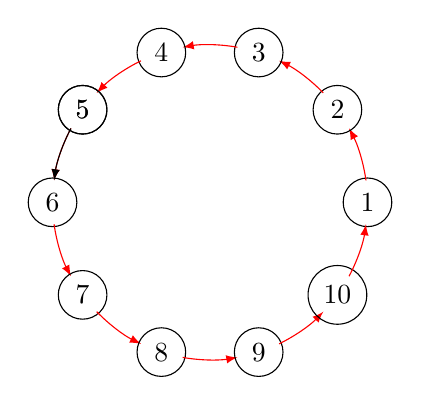
\begin{tikzpicture}

\def \n {10}
\def \radius {2cm}
\def \margin {8} % margin in angles, depends on the radius

\foreach \s in {1,...,10}
{
  \node[draw, circle] at ({360/\n * (\s - 1)}:\radius) {$\s$};
  \draw[->, >=latex, red] ({360/\n * (\s - 1)+\margin}:\radius)
    arc ({360/\n * (\s - 1)+\margin}:{360/\n * (\s)-\margin}:\radius);
}
  \node[draw, circle] at ({360/\n * (5 - 1)}:\radius) {$5$};
  \draw[->, >=latex] ({360/\n * (5 - 1)+\margin}:\radius)
    arc ({360/\n * (5 - 1)+\margin}:{360/\n * (5)-\margin}:\radius);

\end{tikzpicture} & \tikzset{main node/.style={circle,fill=white!20,draw,minimum size=0.5cm,inner sep=0pt},}
\usetikzlibrary{graphs,graphs.standard}

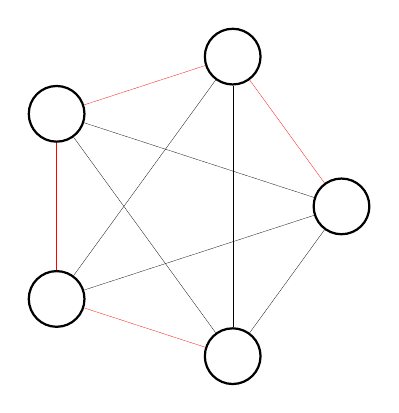
\begin{tikzpicture}
  \foreach \x in {1,...,5}{%
    \pgfmathparse{(\x-1)*360/5}
    \node[draw,circle,inner sep=0.25cm] (N-\x) at (\pgfmathresult:2.0cm) [thick] {};
  }
  \pgfmathparse{7*360/5}
  %\node[circle,red] (N-8) at (\pgfmathresult:5.4cm) {\ldots};
  
  \path (N-1) edge[ultra thin,-, red] (N-2);
  \path (N-2) edge[ultra thin,-, red] (N-3);
  \path (N-3) edge[ultra thin,-, red] (N-4);
  \path (N-4) edge[ultra thin,-, red] (N-5);
  
  \path (N-1) edge[ultra thin,-] (N-3);
  \path (N-1) edge[ultra thin,-] (N-4);
  \path (N-1) edge[ultra thin,-] (N-5);
  
  \path (N-2) edge[ultra thin,-] (N-4);
  \path (N-2) edge[ultra thin,-] (N-5);
  
  \path (N-3) edge[ultra thin,-] (N-5);
  
\end{tikzpicture} \\
\end{tabular}
    
    
    
\pagebreak
\subsubsection{Performance}
%actualizar grafico%
En esta secci\'on utilizaremos lo mencionado en los tests: Vamos a comparar que diferencia hay entre dos grafos que tienen la misma cantidad de aristas, difieran ampliamente en la cantidad de vertices y que ademas, las  $n-1$ aristas mas pesadas, sean las que efectivamente conforman nuestro AGM. Con esto ultimo logramos que el algoritmo de Kruskal corte mucho antes de tener que recorrer todas las aristas del grafo.
Esta idea la conceptualizamos en el siguiente gr\'afico, en el cu\'al se observa que la cantidad de aristas que revisa el algoritmo de Kruskal es mucho mayor para el grafo donde, a misma cantidad de aristas, menor cantidad de vertices.\\

\begin{figure}[h!]
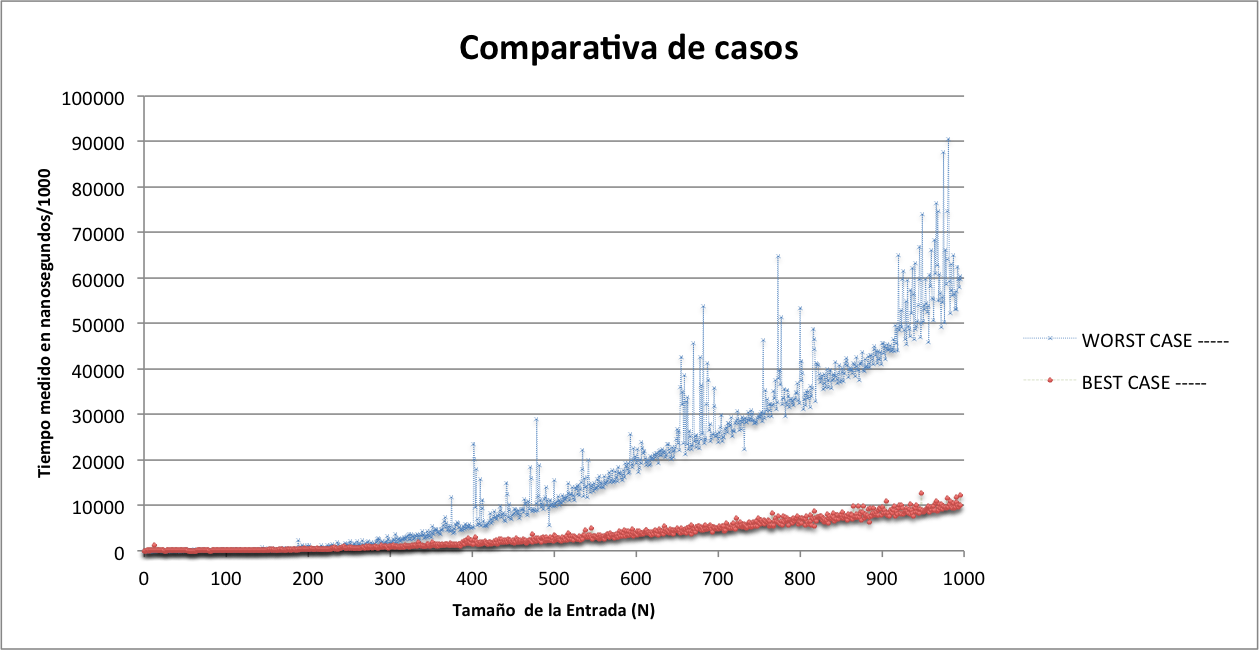
\includegraphics[width=140mm]{ej3-comp-tp2.png}
\centering
\caption{Tiempo de ejecuci\'on en funci\'on de la cantidad de aristas.}
\label{overflow3}
\end{figure}

\pagebreak
Luego decidimos ver que sucedia si no elegiamos las aristas del k5 para estar en un mejor caso y decidimos hacer que los pesos que se le asigaban fuesen random. En el siguiente grafico se observan cosas interesantes, como puede ser que hay dos o tres casos en el cual el random de pesos cayo en el mejor caso, pero tambien vemos que es muy particular ya que la mayoria de casos se mantienen con el crecimiento de la complejidad. 
\begin{figure}[h!]
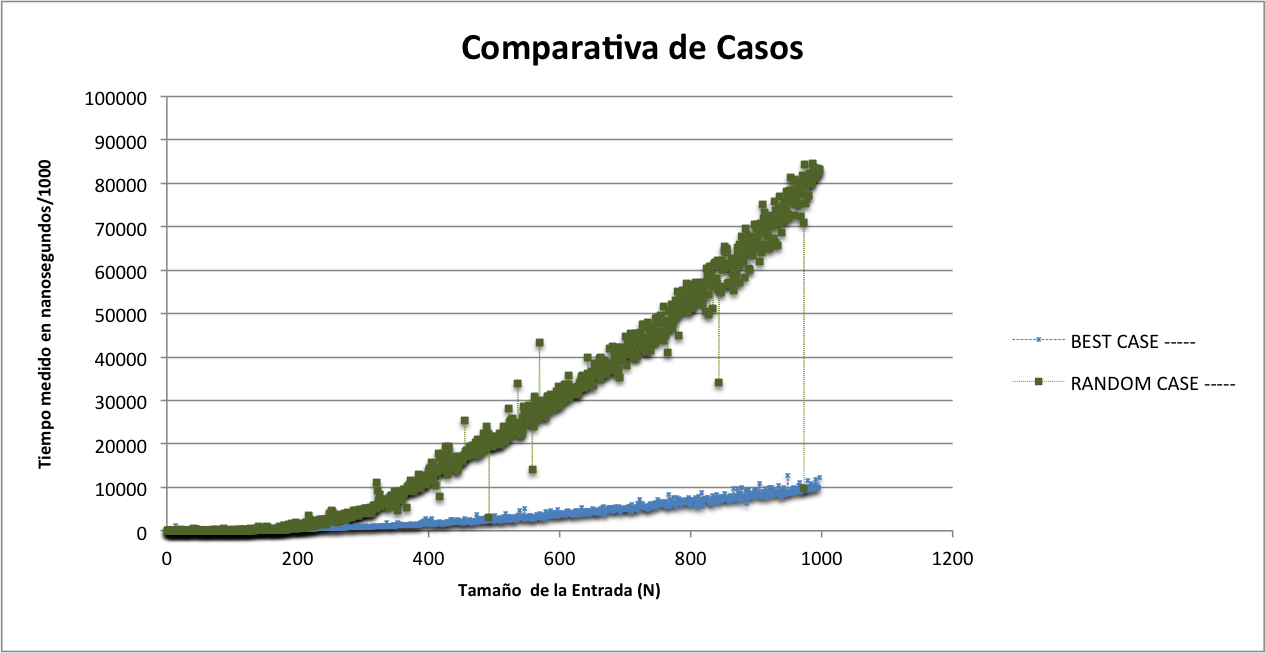
\includegraphics[width=140mm]{ej3-comp2-tp2.png}
\centering
\caption{Tiempo de ejecuci\'on en funci\'on de la cantidad de aristas.}
\label{overflow3}
\end{figure}

Hay tres picos en las medici\'ones del caso random, esto lo consideramos como ruido de la virtual machine de java en la que corrieron nuestros tests.

